\documentclass[10pt,twocolumn]{article}
\usepackage[T1]{fontenc}
\usepackage[utf8]{inputenc}
\usepackage{lmodern,microtype}
\usepackage[letterpaper,margin=.70in,columnsep=.25in]{geometry}
\usepackage{amsmath,amssymb,mathtools}
\usepackage{booktabs,tabularx,array}
\usepackage{enumitem}
\usepackage{xcolor,tikz}
\usetikzlibrary{arrows.meta,positioning,fit,shapes.geometric}
\usepackage{titlesec}
\usepackage{balance}
\usepackage{float}
\usepackage{hyperref}
\definecolor{ink}{HTML}{17354B}
\definecolor{accent}{HTML}{087B86}
\definecolor{soft}{HTML}{EDF4F5}
\definecolor{quiet}{HTML}{4C616C}
\hypersetup{colorlinks=true,linkcolor=ink,citecolor=accent,urlcolor=accent,
 pdfauthor={Yossi Eliaz},
 pdftitle={Evidence Frontiers: Physics-Guided Speculative Sandboxes for Agentic Development}}
\setlength{\parindent}{0pt}
\setlength{\parskip}{2.65pt}
\raggedbottom
\setlength{\abovedisplayskip}{4pt}
\setlength{\belowdisplayskip}{4pt}
\renewcommand{\arraystretch}{1.1}
\setlist[itemize]{leftmargin=*,topsep=3pt,itemsep=1pt,parsep=0pt}
\titleformat{\section}{\large\bfseries\color{ink}}{\thesection}{.45em}{}
\titleformat{\subsection}{\normalsize\bfseries\color{ink}}{\thesubsection}{.5em}{}
\titlespacing*{\section}{0pt}{10pt}{4pt}
\titlespacing*{\subsection}{0pt}{7pt}{2pt}
\newcommand{\Pp}{\mathbb P}
\newcommand{\Ee}{\mathbb E}
\newcommand{\TV}{\operatorname{TV}}
\newcommand{\Anc}{\operatorname{Anc}}
\newcommand{\head}[1]{\textbf{\color{ink}#1}}
\newcommand{\claim}[1]{\textbf{\color{accent}#1}}
\title{\vspace{-1.4em}\textcolor{ink}{\bfseries Evidence Frontiers}\\[-.5ex]
\large Physics-Guided Speculative Sandboxes for Agentic Development}
\author{Yossi Eliaz\\[-2pt]\small Cambridge SRG seminar research companion \;\textbar\; 13 October 2026\\[-3pt]
\small\href{https://github.com/zozo123/cam-talk-london-26}{Cambridge repository}\;\textbar\;
\href{https://arxiv.org/abs/2607.09689}{Evidence-aware reduction}}
\date{}
\begin{document}
\maketitle\vspace{-1.1em}
\begin{abstract}\noindent
Forkable execution makes it possible to compute futures before their premises have been verified. The systems problem is not creating more branches: it is choosing which dependencies to execute ahead, which hypotheses to distinguish, and when their results merit promotion. We propose \emph{evidence frontiers}: an executable DAG may advance speculatively while a controller-owned frontier advances only across trustworthy, artifact-bound checks. We connect the scheduler to expected accepted prefixes in speculative decoding, committor probabilities in transition-path theory, value of information, rare-event splitting, and common-random-number experimental design. The key distinction is that correlation can \emph{help} causal comparisons yet \emph{hurt} independent-evidence claims. We derive simple economic and statistical decision rules, specify an end-to-end protocol and falsifiable benchmarks, and audit the mathematics with a dependency-free script. This is a research design, not a measured integrated sandbox runtime.
\end{abstract}
\vspace{-0.5em}

\section{The problem: optimize the critical path, not the fork count}

The Cambridge factory case shows the danger of optimizing an attractive but irrelevant number. One measured serial repair run spent $20.3$\,s in initial setup and $2{,}557.517$\,s of recorded stage time: setup was only $0.794\%$. An imagined $100\times$ setup speedup saves about $20.1$\,s, not an order of magnitude overall. Its parallel edit-node critical path was a \emph{calculation}, not an observed fork run; warm worktrees can also exploit file-level parallelism \cite{cam}. The runtime should compete against a \emph{warm} alternative using time and money \emph{to a verified result}, not create latency in isolation.

\claim{Proposed abstraction: two frontiers.} A private \emph{execution frontier} may run downstream of a provisional patch. A \emph{trusted evidence frontier} only crosses a transition after an external checker validates its declared obligations on the exact artifact. A child may draft, but cannot edit the oracle, sign its own receipt, inherit publication authority, or unsend an external effect. This is CPU reorder-buffer thinking applied to agentic work, but not a first claim to speculation: Sherlock already overlaps downstream execution with verification \cite{sherlock}. We ask \emph{where to fork, what to learn, and what the results prove}.

\begin{figure}[t]
\centering
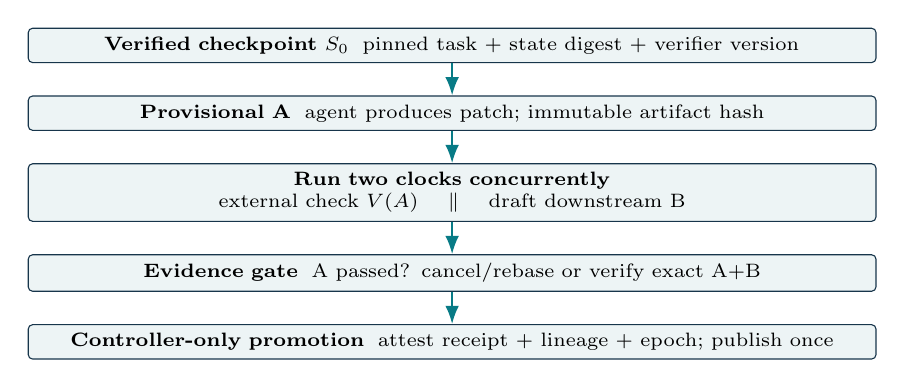
\begin{tikzpicture}[font=\scriptsize,>=Latex,
 node distance=4.1mm,
 box/.style={draw=ink,fill=soft,rounded corners=1.6pt,align=center,inner sep=3.1pt,text width=.87\columnwidth},
 arrow/.style={-Latex,thick,draw=accent}]
\node[box] (root) {\textbf{Verified checkpoint $S_0$}\; pinned task + state digest + verifier version};
\node[box,below=of root] (patch) {\textbf{Provisional A}\; agent produces patch; immutable artifact hash};
\node[box,below=of patch] (fork) {\textbf{Run two clocks concurrently}\\ external check $V(A)$ \quad $\parallel$ \quad draft downstream B};
\node[box,below=of fork] (gate) {\textbf{Evidence gate}\; A passed? cancel/rebase or verify exact A+B};
\node[box,below=of gate] (out) {\textbf{Controller-only promotion}\; attest receipt + lineage + epoch; publish once};
\draw[arrow] (root)--(patch);\draw[arrow] (patch)--(fork);\draw[arrow] (fork)--(gate);\draw[arrow] (gate)--(out);
\end{tikzpicture}
\caption{Execution can outrun evidence; publication cannot. External tool effects must be fenced \emph{before} dispatch.}
\end{figure}

\section{Which kind of speculation? Three different jobs}

\begin{table}[t]\centering\footnotesize
\begin{tabularx}{\columnwidth}{@{}p{.21\columnwidth}X@{}}\toprule
Mode & Optimization target and hazard\\\midrule
\textbf{Run ahead} & Hide verification latency by executing a dependent continuation. A rejected ancestor invalidates descendants.\\
\textbf{Portfolio} & Find at least one verified solution. Overlapping failure modes make replicas redundant.\\
\textbf{Paired trial} & Compare interventions under matched conditions; shared environmental noise can \emph{improve} precision.\\\bottomrule
\end{tabularx}\caption{A common snapshot does not imply the same objective or evidence rule.}
\end{table}

These are not equivalent. A portfolio has an \emph{OR} objective across alternative final artifacts. Run-ahead has an \emph{AND} dependency along one executable path. Paired trials estimate a \emph{difference}. Choosing the wrong mathematics for a mode leads either to wasted compute or false confidence.

\section{What transfers from speculative decoding?}

For target token law $p$ and cheap proposal $q$, exact speculative sampling accepts $x\sim q$ with $a(x)=\min\{1,p(x)/q(x)\}$ for $q(x)>0$. Averaging gives
\begin{equation}\label{eq:tv}
\alpha_{\rm tok}=\sum_x \min\{p(x),q(x)\}=1-\TV(p,q).
\end{equation}
A residual draw from $[p-q]_+/\TV(p,q)$ upon rejection restores the exact target distribution \cite{leviathan}. In contrast, passing a software checker has no such correction theorem; even an independently controlled test suite may miss a wrong patch. EAGLE-2 and OPT-Tree motivate \emph{context-dependent proposal trees}, not distribution-preservation guarantees for agent code \cite{eagle2,opttree}.

For $D$ dependent speculative transitions, let $L$ be the number of consecutive successfully checked transitions. For the true joint verifier events $A_j$,
\begin{equation}\label{eq:prefix}
\Ee[L]=\sum_{j=1}^{D}\Pp(A_1\cap\cdots\cap A_j).
\end{equation}
This tail-sum identity is exact; it does not assume independent checks. Yet equal-length prefixes need not have equal value: one transition may save an hour, another milliseconds. We should maximize \emph{verified critical-path progress per unit cost}, not accepted-step count.

\subsection{A Jeff-Dean-style crossover calculation}
Suppose draft A takes $d_A$, checking A takes $v$, and follow-up draft B takes $d$; final checking costs $v_f$. If A passes and the resources do not contend:
\begin{align}
T_{\rm serial}&=d_A+v+d+v_f,\\
T_{\rm ahead}&=d_A+\max\{v,d\}+v_f,\\
\Delta T_{\rm pass}&=\min\{v,d\}.\label{eq:overlap}
\end{align}
Let $a=\Pp(A\text{ passes})$, $h$ be added wall-time overhead, $c_B$ the cost of speculatively drafting B, $c_f$ extra fork/coordination compute, $\beta$ the value of a second saved and $\lambda$ the price of compute. Under this deliberately idealized two-path model---no contention, no latency penalty if A fails, and no reusable B after failure---run-ahead is worthwhile if
\begin{equation}\label{eq:threshold}
\boxed{\beta\,a\min\{v,d\}>\beta h+\lambda[(1-a)c_B+c_f].}
\end{equation}
The left side is expected hidden waiting; the right charges overhead and wasted speculation. Example: $d_A=10,v=30,d=20,v_f=30$ seconds gives $90\to70$ seconds \emph{conditional on A passing}; with $a=.8$, the ideal expected gross saving is $16$ seconds, and the wasted B work is $4$ worker-seconds when $c_B=20$ worker-seconds. These are illustrations, \emph{not} measurements.

\claim{Queueing changes the answer.} A verifier with mean service demand $\Ee[V]$ and long-run arrival rate $\lambda_v$ has utilization $\rho_v=\lambda_v\Ee[V]$ for one equivalent server. A stable stationary queue requires $\rho_v<1$; launching more branches can saturate the \emph{verifier}, making both cost and latency worse. The scheduler needs the verifier's shadow price and tail latency, not just its throughput \cite{tail}.

\section{Physics suggests predicting destinations, not next checks}

\subsection{The committor: eventual verified success}
For a complete Markov state $s$ under a \emph{fixed} continuation policy $\pi$, define the committor
\begin{equation}\label{eq:committor}
h_\pi(s)=\Pp_\pi(\tau_G<\tau_F\mid S_0=s),
\end{equation}
where $G$ is verified goal completion and $F$ is terminal failure. With transition kernel $P_\pi(s'|s)$,
\begin{equation}\label{eq:harmonic}
 h_\pi(s)=\sum_{s'}P_\pi(s'|s)h_\pi(s'),
 \quad h_\pi|_G=1,\quad h_\pi|_F=0.
\end{equation}
This is the committor equation from transition-path theory \cite{tpt}. A branch can fail its next superficial check yet be useful because it discovers a reproducer or root cause; conversely, a patch can pass easy checks while having little chance of eventual success. An \emph{estimated} committor can rank states by expected future value, but it is policy-specific and must be validated out of sample.

There is a mathematically exact analogy worth keeping \emph{separate} from software correctness: if $h$ is the true positive harmonic committor for a Markov process, the Doob transform
\begin{equation}\label{eq:doob}
P^h(s'|s)=P(s'|s)\frac{h(s')}{h(s)}
\end{equation}
constructs the process conditioned on reaching $G$ before $F$ (on appropriate nonabsorbing states). This is \emph{not} an executable correctness guarantee for agents with unknown transitions; replacing $h$ by a learned score gives a \emph{heuristic proposal policy}, not a valid exact conditioning theorem.

\subsection{Rare-event splitting: fork where progress persists}
Suppose success requires nested milestones $E_m\subseteq\cdots\subseteq E_1$, with positive conditioning probabilities. Then
\begin{equation}\label{eq:split}
\Pp(E_m)=\prod_{k=1}^m\Pp(E_k\mid E_{k-1}),
\quad E_0=\Omega.
\end{equation}
Adaptive multilevel splitting retains trajectories reaching promising levels and resamples continuations instead of repeatedly paying for the entire prefix \cite{ams}. In coding, plausible \emph{candidate milestones} are reproducer, root cause, targeted behavioral fix, integration check and final review. But a checkpoint is reusable only when its state is valid for the next intervention. Blindly cloning a flawed hypothesis creates genealogical collapse, not progress.

\claim{Discovery is not probability estimation.} Retaining high-score trajectories changes the sampling law from $P$ to $Q$. To estimate an event's \emph{original} probability under a valid importance-sampling setup requires
\begin{equation}\label{eq:iw}
\Pp_P(G)=\Ee_Q\!\left[\frac{dP}{dQ}\,\mathbf1_G\right],\quad P\ll Q.
\end{equation}
Without a justified likelihood ratio or a valid rare-event estimator, optimized branch populations cannot claim calibrated original frequencies. The same caution applies to evidence-aware statistical reduction.

\section{The most useful fork may be a diagnostic test}

Probability of passing the \emph{next} check ignores the information gained from a failure. Suppose two root causes have probability $1/2$ each, each corresponding repair costs 10 units, and a perfect discriminating diagnostic costs 2. Blindly try repair A, then B if needed:
\[
\Ee[C_{\rm repairs}]=10+\tfrac12(10)=15.
\]
Diagnose first and make the correct repair:
\[
\Ee[C_{\rm diagnostic}]=2+10=12.
\]
The test produces no patch yet saves three expected cost units. It has \emph{value of information} (VOI).

With current information $H$, candidate terminal action $a$, experiment $e$ with result $O_e$, utility $U$, and experiment cost $C(e),$
\begin{equation}\label{eq:voi}
\begin{aligned}
\mathrm{VOI}(e)={}&\Ee_{O_e\mid H}\!\left[\max_a\Ee[U(a)\mid H,O_e]\right]\\[-1pt]
&-\max_a\Ee[U(a)\mid H]-C(e).
\end{aligned}
\end{equation}
The equation describes a single additional observation followed by one terminal decision; richer workflows need dynamic programming. The practical lesson is \emph{schedule tests and interventions together}, not only proposals expected to pass. A deterministic test of the Cambridge \texttt{CellBusy}--same-work-order adoption path might be more valuable than another nearly identical repair attempt \cite{cam}.

\section{The correlation paradox: repeat, diversify, or pair?}

\subsection{Positive correlation can improve paired comparisons}
Assume two matched experiments use the same environmental perturbation $U$:
\begin{equation}\label{eq:paired}
 Y_A=\theta_A+U+\varepsilon_A,\quad
 Y_B=\theta_B+U+\varepsilon_B.
\end{equation}
For mutually independent noise terms with $\operatorname{Var}(U)=\tau^2$ and $\operatorname{Var}(\varepsilon_i)=\sigma^2$, shared-$U$ pairing yields
\begin{equation}\label{eq:variance}
\boxed{\operatorname{Var}(Y_A-Y_B)=2\sigma^2.}
\end{equation}
Independent environmental draws instead yield $2(\tau^2+\sigma^2)$. With $\tau^2=9,\sigma^2=1$, variance goes from $20$ to $2$---a $10\times$ reduction \emph{under this model} \cite{crn}. The general identity is $\operatorname{Var}(A-B)=\operatorname{Var}A+\operatorname{Var}B-2\operatorname{Cov}(A,B)$: pairing helps only when the induced covariance is positive. Reuse identical \emph{test fixtures and controlled input randomness}, never inherited secrets or clone identity/RNG for security.

\subsection{But dependence reduces search coverage}
For a fixed set $S$ of candidate acceptance events $A_i$,
\begin{equation}\label{eq:coverage}
\begin{aligned}
F(S)&=\Pp\!\left(\bigcup_{i\in S}A_i\right),\\
\Delta_j(S)&=F(S\cup\{j\})-F(S)\\[-2pt]
 &=\Pp\!\left(A_j\cap\bigcap_{i\in S}A_i^c\right).
\end{aligned}
\end{equation}
This is monotone and submodular for a \emph{fixed} joint law: new workers have diminishing marginal coverage as the set grows. It does not imply a greedy guarantee for a history-dependent controller. As a counterexample, if exactly one of two mutually exclusive approaches A/B succeeds, then $\Pp(B)=1/2$ yet $\Pp(B\mid A^c)=1$: failure \emph{raises} the other branch's value. Estimate conditional probabilities from held-out family-aware observations, not independence shortcuts.

Finally, in correlated numerical estimation, $K$ equally precise workers with equicorrelation $\rho\geq0$ have
\begin{equation}\label{eq:neff}
 K_{\rm eff}=\frac{K}{1+(K-1)\rho}.
\end{equation}
That result concerns \emph{estimation-error correlation}, not binary patch-success correlation. Shared evidence identifiers and fork lineage are not enough to identify covariance. The previously published reducer rejects declared duplicate IDs but does not fit this covariance model \cite{reduction}.

\section{An implementable controller, not a physics metaphor}

\head{State.} A trusted controller pins $({\tt task,base,manifest,verifier,epoch})$, maintains a directed acyclic graph of provisional artifact hashes, dependency receipts, rejected and censored outcomes, executor costs and effect logs. The policy state also contains a calibrated belief over root-cause hypotheses. Never interpret a timeout as a witnessed test failure.

\head{Safety gates.} Verify capture fidelity and source identity; private writable state; fresh capability/credential issuance; blocked or mediated network/tool effects; budget and resource limits. Copying guest memory does not copy authority. If fidelity or security fails, do not fork. A \emph{warm worktree} must remain a first-class alternative.

\head{Choice.} The action set contains \{diagnose, run ahead, diversify, paired compare, verify now, warm serial, stop\}. For an idealized belief-state controller, the Bellman form is
\begin{equation}\label{eq:bellman}
\begin{aligned}
V(b,s,B)&=\max_{a\in\mathcal A_{\rm safe}(s,B)}\big\{\\[-2pt]
&\quad r_a-\lambda c_a+\Ee_{o\mid b,s,a}
V(b_o,s_o,B-k_a)\big\},
\end{aligned}
\end{equation}
where $b_o,s_o$ are the updated belief and state, $c_a$ is economic cost and $k_a$ consumes budget $B$. Terminal rewards are assigned to an \emph{externally verified} exact artifact. This is a \emph{formulation}, not a solved optimal runtime. A practical heuristic first ranks cheap discriminating tests by VOI, then ranks admissible forks by conditional \emph{marginal} verified progress and potential critical-path savings, rejecting choices with negative net gain or saturated verifier queues. The committor is a learned feature, not an oracle.

\head{Commit.} A child returns bytes, digest and trace; an external, pinned checker issues a controller-authenticated receipt tying \emph{actual} verifier identity to those bytes and to the epoch. Only a current-epoch, fully checked result can move the evidence frontier. Verify the \emph{final composed artifact} after merging patches. Persist artifacts and ledger before teardown, use atomic compare-and-swap on promotion, and block observable tool calls before issue. A green test proves only its stated predicate; repeated search may exploit an incomplete oracle. For illustration, if each of $100$ wrong proposals had an independent $1\%$ false-pass chance, the chance of at least one false pass would be $1-.99^{100}\approx63.4\%$. Real false passes need not be independent; these figures are not a measured bug rate.

\head{Exploration temperature (optional).} For a fixed finite candidate set with prior proposal $q_0(a|s)>0$, maximizing $\Ee_{a\sim\pi}Q(s,a)-T D_{\rm KL}(\pi\Vert q_0)$ yields
\begin{equation}\label{eq:gibbs}
 \pi_T(a|s)\propto q_0(a|s)\exp\{Q(s,a)/T\}.
\end{equation}
Temperature can encourage hypothesis diversity; this is a scheduling \emph{choice}, not an exact-decoding acceptance correction. Reserve exploration budget when the learned committor is uncertain or when repeated failures expose a common-mode hypothesis.

\section{Evaluation: what would change our minds?}

\begin{table}[H]\centering\footnotesize
\begin{tabularx}{\columnwidth}{@{}p{.25\columnwidth}X@{}}\toprule
Question & Required comparison / falsifier \\\midrule
\textbf{Better than warm?} & Warm serial, worktree portfolio, fixed-width forks, adaptive policy; same task, verifier and capped hardware. Reject advantage when warm cost/time dominates.\\
\textbf{Hide waiting?} & Two-stage A$\to$B with A checked concurrently with drafting B. Measure verified critical path, wasted CPU/LLM time, p50/p95, rollback cost and contention.\\
\textbf{Learn from failure?} & Paired diagnostic-first versus direct repair; hold out repo/task families; assess Brier/log loss and decision utility.\\
\textbf{Control error?} & Controlled matched A/B forks versus independent environments; estimate paired covariance and confidence coverage across \emph{independent} families.\\
\textbf{Trust gate?} & Challenge stale epochs, tampered checkers, duplicate evidence, unverified merged bytes and speculative observable tool calls.\\\bottomrule
\end{tabularx}\caption{Proposed experiments; none are claimed executed.}
\end{table}

\head{Design discipline.} Preserve the Cambridge preregistered Gate~0, H1 warm-cache test, and H2 sibling-coupling test \emph{unchanged} \cite{cam}. This note proposes a separate exploratory follow-up. Report all attempted tasks, partial failures, timeouts, rejected branches, policy propensities and held-out correctness checks. Failure to beat a warm baseline is a meaningful result. Use falsifying examples where more forks increase verifier load or where repeated testing finds a false pass. Exact success labels for semantic correctness require a genuinely stronger hold-out oracle, not the same suite repeatedly queried.

\section*{Conclusion: a compiler for experiments}
\noindent\colorbox{soft}{\parbox{.945\columnwidth}{\vspace{4pt}\small\textbf{Fork only when reached state is valid and reuse beats warm reconstruction.}\par
\textbf{Execute ahead to remove waiting; diversify to increase coverage; pair to isolate causal effects.}\par
\textbf{Spend the next unit of compute where its marginal verified progress \emph{or information gain} is highest.}\par
\textbf{Promote exact bytes once; let only justified evidence increase confidence.}\vspace{4pt}}}

\begin{thebibliography}{11}\footnotesize\setlength{\itemsep}{1pt}
\bibitem{cam} Y. Eliaz, \href{https://github.com/zozo123/cam-talk-london-26}{\emph{Forkable Sandboxes: Cambridge Seminar}}, 2026; \texttt{CLAIM-FENCE.md}, \texttt{PREREGISTRATION.md}.
\bibitem{reduction} Y. Eliaz, \href{https://arxiv.org/abs/2607.09689}{\emph{Evidence-Aware Reduction for Forkable Compute}}, arXiv:2607.09689v4, 2026.
\bibitem{leviathan} Y. Leviathan, M. Kalman, Y. Matias, \href{https://proceedings.mlr.press/v202/leviathan23a.html}{\emph{Fast Inference from Transformers via Speculative Decoding}}, ICML 2023.
\bibitem{eagle2} Y. Li et al., \href{https://aclanthology.org/2024.emnlp-main.422/}{\emph{EAGLE-2: Faster Inference of Language Models with Dynamic Draft Trees}}, EMNLP 2024.
\bibitem{opttree} J. Wang et al., \href{https://aclanthology.org/2025.tacl-1.8/}{\emph{OPT-Tree: Speculative Decoding with Adaptive Draft Tree Structure}}, TACL 2025.
\bibitem{sherlock} Y. Ro et al., \href{https://www.microsoft.com/en-us/research/publication/sherlock-reliable-and-efficient-workflow-execution/}{\emph{Sherlock: Reliable and Efficient Workflow Execution}}, Microsoft Research, 2025.
\bibitem{tail} J. Dean, L. A. Barroso, \href{https://research.google/pubs/the-tail-at-scale/}{\emph{The Tail at Scale}}, CACM 2013.
\bibitem{tpt} W. E, E. Vanden-Eijnden, \href{https://doi.org/10.1146/annurev.physchem.040808.090412}{\emph{Transition-Path Theory and Path-Finding Algorithms for the Study of Rare Events}}, Annu. Rev. Phys. Chem. 2010.
\bibitem{ams} C.-E. Br\'ehier et al., \href{https://doi.org/10.1214/16-AAP1185}{\emph{Unbiasedness of Some Generalized Adaptive Multilevel Splitting Algorithms}}, Ann. Appl. Probab. 2016.
\bibitem{crn} J. P. C. Kleijnen, \href{https://doi.org/10.1287/mnsc.34.1.65}{\emph{Analyzing Simulation Experiments with Common Random Numbers}}, Management Science, 1988.
\end{thebibliography}
\end{document}
